\section{Results}
\label{sec-results}

\begin{figure*}[t]
       \begin{center}
                       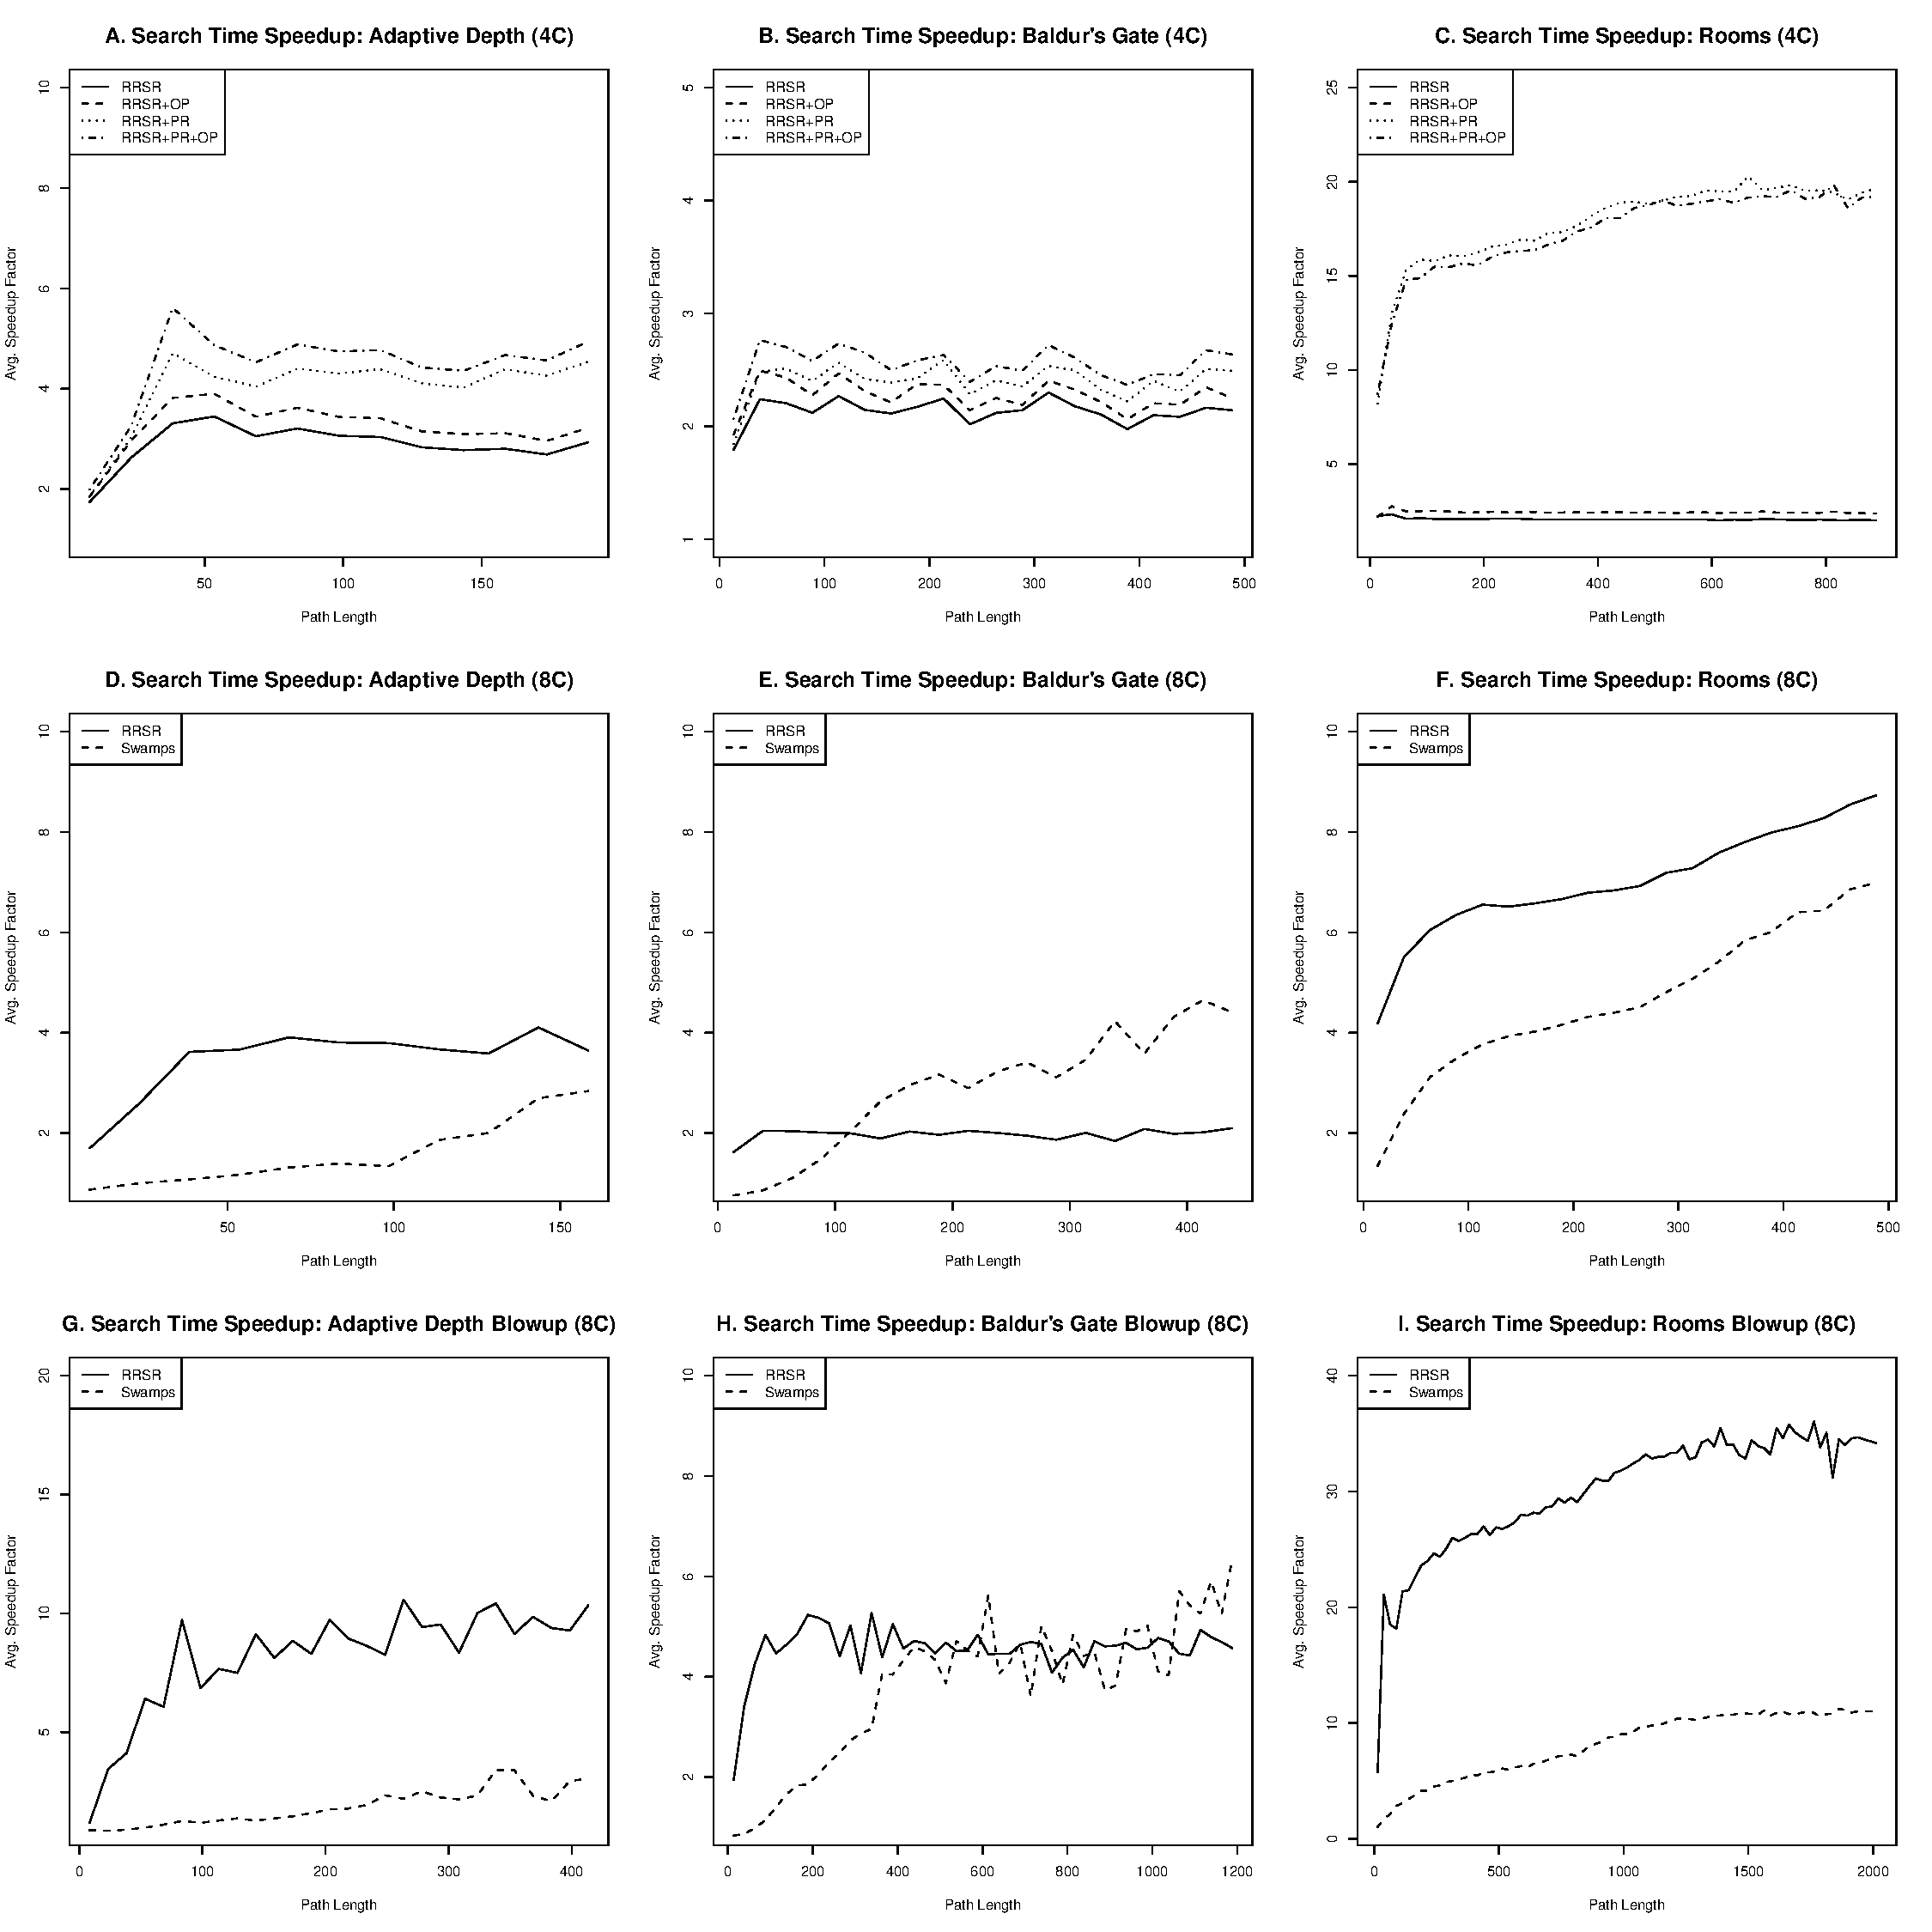
\includegraphics[width=1.95\columnwidth, trim = 10mm 10mm 10mm 0mm]{diagrams/speedup.pdf}
       \end{center}
       \caption{Average A* speedup on each of our three benchmarks. 
		Results are given in terms of nodes expanded and search time.}
\label{fig-speedup}
\end{figure*}

Our main results are given in Table \ref{table-graphsize}, Table
\ref{table-speedup} and Figure \ref{fig-speedup}.
We will briefly introduce each and then discuss them in the context
of our three benchmarks.
\par
Table \ref{table-graphsize} measures the size of our modified grid maps.
We give figures for the average number of nodes and average number of edges
as a proportion of the number of nodes and edges in the original grid maps
from each benchmark.


\input graphsize_table

Some text introducing the speedup table.
\input speedup_table


